\documentclass[11pt]{article}

% ACL/EMNLP style compatible
\usepackage[utf8]{inputenc}
\usepackage[T1]{fontenc}
\usepackage{amsmath,amssymb}
\usepackage{booktabs}
\usepackage{graphicx}
\usepackage{xcolor}
\usepackage{hyperref}
\usepackage{multirow}
\usepackage{tablefootnote}
\usepackage[margin=1in]{geometry}
\usepackage{caption}
\usepackage{subcaption}
\usepackage{enumitem}

\definecolor{highlight}{RGB}{220,50,47}

\title{\textbf{TreeBench: A Benchmark for Hierarchy-Sensitive Retrieval\\over Structured Regulatory Corpora}}

\author{
  Sahil Soni\\
  Independent Researcher\\
  \texttt{sahil.soni2409@gmail.com}
}

\date{}

\begin{document}

\maketitle

\begin{abstract}
Retrieval-augmented generation (RAG) systems are increasingly deployed over hierarchically structured corpora such as legal codes, tax regulations, and compliance frameworks. We introduce \textbf{TreeBench}, a benchmark of 861 questions designed to expose \emph{structural evidence failures}---cases where semantically similar text exists at multiple positions in a document tree, but only one position carries legal authority for a given query. TreeBench operationalizes 10 failure modes (override chains, scope disambiguation, cross-references, etc.) across 5 regulatory domains mined from the U.S.\ Electronic Code of Federal Regulations. We evaluate 8 retrieval and reasoning methods and find a striking gap: the best non-oracle method achieves 76\% answer accuracy but only 45\% required-node recall, meaning it produces correct-\emph{looking} answers while missing the structural evidence that authorizes them. Chain-of-thought prompting and LLM-as-judge verification do not recover this missing evidence because the failure is upstream of reasoning---in context selection. In our evaluated setting, reranking worsens performance by amplifying structural confounders. We release TreeBench as an open challenge: no evaluated method recovers the full structural authority path.\footnote{Dataset, code, and evaluation scripts: \url{https://github.com/whitepaper27/TreeBench}}
\end{abstract}


% ════════════════════════════════════════════════════════════════════
\section{Introduction}
\label{sec:intro}

Retrieval-augmented generation has become the standard architecture for question answering over large document collections \cite{lewis2020rag}. The implicit assumption is that \emph{semantic similarity} is a reliable proxy for \emph{relevance}: if a retrieved passage is ``about'' the query topic, it contains the information needed to answer.

This assumption breaks down in hierarchically structured corpora. Legal codes, tax regulations, medical guidelines, and compliance frameworks organize provisions in trees where \emph{position determines authority}. A general rule at depth 3 may be overridden by a specific exception at depth 6. Two sibling sections may define the same term differently for different contexts. A cross-reference at one node may point to a controlling provision in an entirely different subtree. In all these cases, the retrieval problem is not semantic relevance---it is \textbf{authority selection}.

We identify a class of failure we call \textbf{structural confounder pairs}: two nodes in a document tree that are semantically similar (high cosine similarity in embedding space) but structurally incompatible (only one is authoritative for a given query). Standard embedding-based retrieval cannot distinguish them. Only tree position resolves the correct answer.

To measure this failure systematically, we introduce \textbf{TreeBench-861}, a benchmark of 861 questions spanning 5 regulatory domains and 10 structural failure types, constructed from the U.S.\ Electronic Code of Federal Regulations (eCFR). Each question is annotated with:
\begin{itemize}[nosep]
    \item A \textbf{gold answer} derivable only from the correct structural path
    \item \textbf{Required node IDs}---the minimum set of tree nodes needed as evidence
    \item \textbf{Distractor node IDs}---structurally confounding nodes that similarity-based retrieval is likely to surface
    \item The \textbf{gold path} through the tree hierarchy
\end{itemize}

This annotation structure enables metrics beyond answer accuracy: we measure \textbf{required-node recall} (did the system retrieve the structural evidence?) and \textbf{path accuracy} (did it find the correct position in the tree?). These metrics reveal a gap invisible to accuracy alone.

Our key findings:
\begin{enumerate}[nosep]
    \item The task is fully answerable: an oracle achieves 100\% on all metrics.
    \item BM25 and hybrid retrieval reach 76\% answer accuracy but only 45\% required-node recall. They produce correct answers for the wrong structural reasons.
    \item Chain-of-thought reasoning (72\% accuracy) and LLM-as-judge verification (57\% accuracy) do not improve recall beyond dense RAG's 34\%, because reasoning cannot recover evidence that retrieval never surfaced.
    \item In our evaluated setting, neural reranking \emph{worsens} performance (36\% accuracy, 21\% recall) by amplifying the very confounders the benchmark targets.
    \item Naive tree traversal achieves only 2\% accuracy, establishing that structure-aware navigation remains an open challenge.
\end{enumerate}

TreeBench demonstrates that \textbf{answer accuracy alone is an insufficient evaluation metric for retrieval over structured corpora}. A system can appear to work (76\% accuracy) while systematically failing to recover the evidence that would make its answers legally defensible.


% ════════════════════════════════════════════════════════════════════
\section{Related Work}
\label{sec:related}

\paragraph{Retrieval-augmented generation.} RAG systems combine retrieval with generation to answer questions over large corpora \cite{lewis2020rag, gao2024ragsurvey}. Standard benchmarks such as Natural Questions \cite{kwiatkowski2019nq}, TriviaQA \cite{joshi2017triviaqa}, and MS MARCO \cite{nguyen2016msmarco} evaluate retrieval primarily through downstream answer accuracy. These benchmarks assume flat document collections where any passage containing the answer is equally valid evidence. Recent domain-specific benchmarks like FinanceBench \cite{islam2024financebench} evaluate RAG over specialized corpora but do not isolate the structural authority dimension.

\paragraph{Structured and hierarchical QA.} Prior work has explored question answering over structured data including knowledge graphs, tables, and multi-hop reasoning over flat document sets \cite{yang2018hotpotqa}. GraphRAG \cite{edge2024graphrag} introduces graph-based indexing for summarization, and TreeRAG \cite{tao2025treerag} proposes hierarchical storage for long-document retrieval. However, neither addresses the hierarchical authority selection problem where tree position---not content---determines which provision controls. Unlike these, TreeBench specifically targets this failure mode.

\paragraph{Legal NLP.} Legal retrieval benchmarks such as LegalBench \cite{guha2023legalbench}, CUAD \cite{hendrycks2021cuad}, and CaseHOLD \cite{zheng2021casehold} focus on legal reasoning capabilities. Recent work has begun benchmarking RAG specifically for legal QA \cite{pipitone2024legalbenchrag}, but these evaluate whether a model can interpret legal language correctly, assuming the relevant provision has been identified. TreeBench complements this work by evaluating whether the relevant provision can be \emph{found} when structural confounders exist.

\paragraph{Retrieval techniques.} BM25 \cite{robertson2009bm25} remains a strong baseline for lexical retrieval. Dense passage retrieval \cite{karpukhin2020dense} using sentence embeddings \cite{reimers2019sentencebert, wang2020minilm} has become the dominant neural approach. Neural reranking \cite{nogueira2020reranking} and chain-of-thought prompting \cite{wei2022cot} have been proposed to improve retrieval and reasoning quality, respectively. Liu et al.\ \cite{liu2024lostmiddle} show that LLMs struggle with evidence positioned in the middle of long contexts; our findings reveal a complementary failure: models cannot reason over evidence that retrieval never surfaced. Our results show that these techniques do not address---and in the case of reranking, can exacerbate---structural authority failures in hierarchical corpora.

\paragraph{Evidence attribution.} Recent work on attribution \cite{rashkin2023attribution} evaluates whether generated text is supported by cited evidence. TreeBench goes further: it evaluates whether the \emph{correct} evidence was retrieved, distinguishing authoritative from merely relevant sources.


% ════════════════════════════════════════════════════════════════════
\section{The TreeBench Benchmark}
\label{sec:benchmark}

\subsection{Design Principles}

TreeBench is designed around three principles:

\begin{enumerate}[nosep]
    \item \textbf{Structural authority, not semantic relevance.} Each question has a structural confounder: a node that is semantically similar to the correct answer but structurally incorrect. Retrieval systems that rely solely on similarity will surface the confounder.
    \item \textbf{Evidence completeness, not just answer correctness.} Each question requires multiple tree nodes as evidence (mean 2.3 required nodes). A system that guesses the right answer from partial context scores on accuracy but fails on recall.
    \item \textbf{Ecological validity.} Questions are mined from real regulatory text (eCFR) rather than synthetically constructed, preserving the natural complexity of hierarchical legal language.
\end{enumerate}

Table~\ref{tab:examples} illustrates two representative TreeBench questions showing how structural confounders create retrieval failures.

\begin{table*}[t]
\centering
\small
\begin{tabular}{p{1.8cm}p{6.5cm}p{6.5cm}}
\toprule
& \textbf{Example 1: Override Chain} & \textbf{Example 2: Scope Disambiguation} \\
\midrule
\textbf{Domain} & Tax (Title 26) & Finance (Title 12) \\
\textbf{Query} & What are the specific tax liability requirements for corporations under \S~1.11-1? & How is the term ``services'' scoped under the Bank Holding Company Act (\S~225.104)? \\
\textbf{Correct node} & \S~1.11-1(a) at depth 6: specific exceptions for foreign corporations and exempt organizations & \S~225.104(c) at depth 7: definition scoped to ``closely related'' nonbanking activities \\
\textbf{Distractor} & \S~1.11-1(b--d): sibling paragraphs discussing related but non-controlling provisions & \S~225.104(1): a different paragraph defining ``services'' for a separate regulatory context \\
\textbf{Why RAG fails} & General rule and exception share 73\% vocabulary overlap; embedding similarity cannot distinguish parent from overriding child & Both nodes define the same term with near-identical vocabulary; only tree position resolves which scope applies \\
\textbf{Depth} & 6 & 7 \\
\bottomrule
\end{tabular}
\caption{Two representative TreeBench questions. In both cases, the correct and distractor nodes are semantically near-identical; only hierarchical position distinguishes the authoritative provision.}
\label{tab:examples}
\end{table*}

\subsection{Source Corpus}

We use 10 titles from the U.S.\ Electronic Code of Federal Regulations (eCFR), spanning 5 domains:

\begin{table}[h]
\centering
\small
\begin{tabular}{llr}
\toprule
\textbf{Domain} & \textbf{eCFR Titles} & \textbf{Nodes} \\
\midrule
Tax & 26 (Internal Revenue), 31 (Treasury) & 187,451 \\
Finance & 12 (Banks), 17 (Securities) & 112,809 \\
Medical & 21 (Food \& Drugs), 42 (Public Health) & 138,622 \\
Legal & 29 (Labor), 15 (Commerce) & 89,441 \\
Compliance & 40 (Environment), 45 (HHS/HIPAA) & 63,470 \\
\midrule
\textbf{Total} & \textbf{10 titles} & \textbf{591,793} \\
\bottomrule
\end{tabular}
\caption{Source corpus: 10 eCFR titles parsed into tree nodes across 5 regulatory domains.}
\label{tab:corpus}
\end{table}

Each title is parsed into a tree structure preserving the eCFR's hierarchical organization (Title $\to$ Chapter $\to$ Subchapter $\to$ Part $\to$ Subpart $\to$ Section $\to$ Paragraph). The resulting 591,793 nodes form the retrieval corpus.

\subsection{Failure Taxonomy}
\label{sec:taxonomy}

We define 10 structural failure types that capture distinct mechanisms by which position-agnostic retrieval fails. Table~\ref{tab:taxonomy} presents the full taxonomy.

\begin{table*}[t]
\centering
\small
\begin{tabular}{clllp{5.5cm}}
\toprule
\textbf{\#} & \textbf{Failure Type} & \textbf{Signal} & \textbf{Confounder} & \textbf{Description} \\
\midrule
1 & Override Chain & except, notwithstanding & parent $\to$ child & Child provision overrides parent rule \\
2 & Scope Disambiguation & same term, 2+ subtrees & sibling & Tree position determines which definition applies \\
3 & Cross-Reference & \S~XXX, ``see section'' & cross-reference & Must follow pointer to controlling provision \\
4 & Conditional Cascade & if\ldots then (nested) & parent $\to$ child & Answer gated by ancestor conditions \\
5 & Temporal Layering & effective dates & temporal & Date qualifier changes applicable rule \\
6 & Sibling Conflict & conflicting shall/shall-not & sibling & Relative position among siblings resolves conflict \\
7 & Definitional Dependency & ``as defined in'' & definition & Term defined in separate subtree \\
8 & Aggregation & ``sum of,'' ``combined'' & cross-reference & Values must be collected from multiple branches \\
9 & Negative Space & coverage gap & missing scope & Correct answer is that no provision exists \\
10 & Depth-Gated Specificity & rate/amount at leaf & parent $\to$ child & Specific value exists only at maximum depth \\
\bottomrule
\end{tabular}
\caption{TreeBench failure taxonomy: 10 structural failure modes that cause position-agnostic retrieval to select the wrong evidence.}
\label{tab:taxonomy}
\end{table*}

\subsection{Construction Pipeline}

The benchmark construction follows a four-stage pipeline (Figure~\ref{fig:pipeline}).

\begin{figure*}[t]
\centering
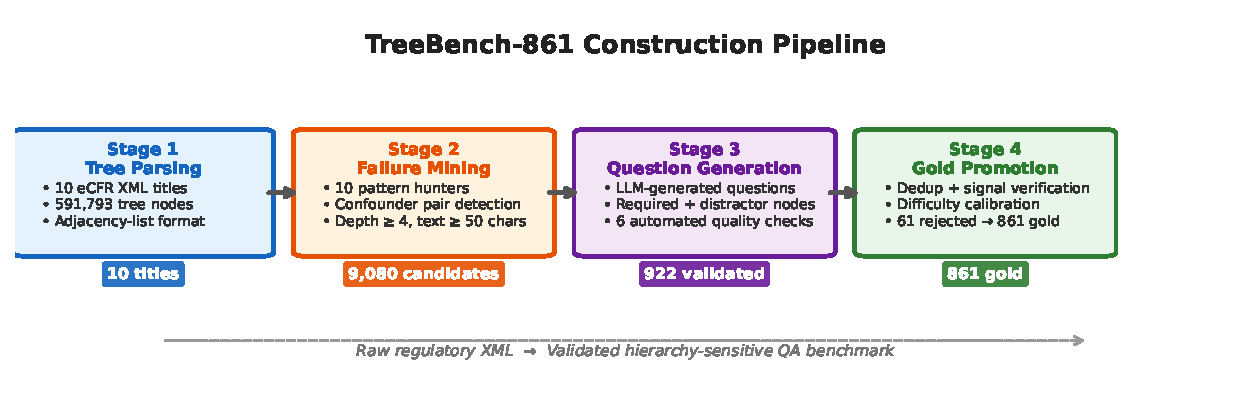
\includegraphics[width=\textwidth]{figures/fig1_pipeline.pdf}
\caption{TreeBench-861 construction pipeline. Raw eCFR XML is parsed into 591,793 tree nodes, mined for 9,080 structural confounder candidates, filtered through LLM-based question generation with 6 automated quality checks, and promoted to 861 gold questions after deduplication and signal verification.}
\label{fig:pipeline}
\end{figure*}

\paragraph{Stage 1: Tree Parsing.} We parse 10 eCFR XML files into adjacency-list tree representations, preserving node types (title, chapter, subchapter, part, subpart, section, paragraph), text content, and hierarchical relationships.

\paragraph{Stage 2: Failure Pattern Mining.} For each failure type, specialized pattern hunters scan the parsed trees for candidate structural confounder pairs nodes that exhibit the failure type's characteristic signal (e.g., ``notwithstanding'' for override chains) at sufficient depth ($\geq$4) with sufficient text ($\geq$50 characters). This yields 9,080 candidate patterns.

\paragraph{Stage 3: Question Generation.} An LLM generates questions from validated candidates using a structured prompt that requires: (a) a question answerable only from the correct structural position, (b) identification of required evidence nodes, (c) identification of distractor nodes, and (d) explanation of why similarity-based retrieval would fail. Generated questions undergo automated validation for quality (no structural giveaways, no signal hallucination, no parser artifacts, no template tails).

\paragraph{Stage 4: Gold Promotion.} Candidates passing all quality checks are promoted to gold status. We enforce diversity (deduplication by question text and evidence overlap) and verify difficulty calibration. The final dataset contains 861 gold questions.

\subsection{Dataset Statistics}

\begin{table}[h]
\centering
\small
\begin{tabular}{lr}
\toprule
\textbf{Statistic} & \textbf{Value} \\
\midrule
Total questions & 861 \\
Domains & 5 \\
Failure types & 10 \\
Domain $\times$ type cells (5$\times$10) & 50 \\
Cells at maximum (20 questions) & 37 \\
\midrule
Difficulty: easy / medium / hard & 207 / 544 / 110 \\
Answer types & 5 \\
\quad numeric / multi-part / classification & 200 / 199 / 195 \\
\quad yes-no / section-reference & 142 / 125 \\
\midrule
Mean tree depth & 5.8 \\
Mean required nodes per question & 2.3 \\
Mean distractor nodes per question & 1.8 \\
Depth range & 4--8 \\
\bottomrule
\end{tabular}
\caption{TreeBench-861 dataset statistics.}
\label{tab:stats}
\end{table}


\subsection{Dataset Validation}

Table~\ref{tab:validation} summarizes automated quality checks applied to the final dataset. We additionally manually inspected a stratified sample of 50 questions (one per domain $\times$ failure-type cell) to verify question readability, evidence alignment, and failure-type assignment.

\begin{figure*}[t]
\centering
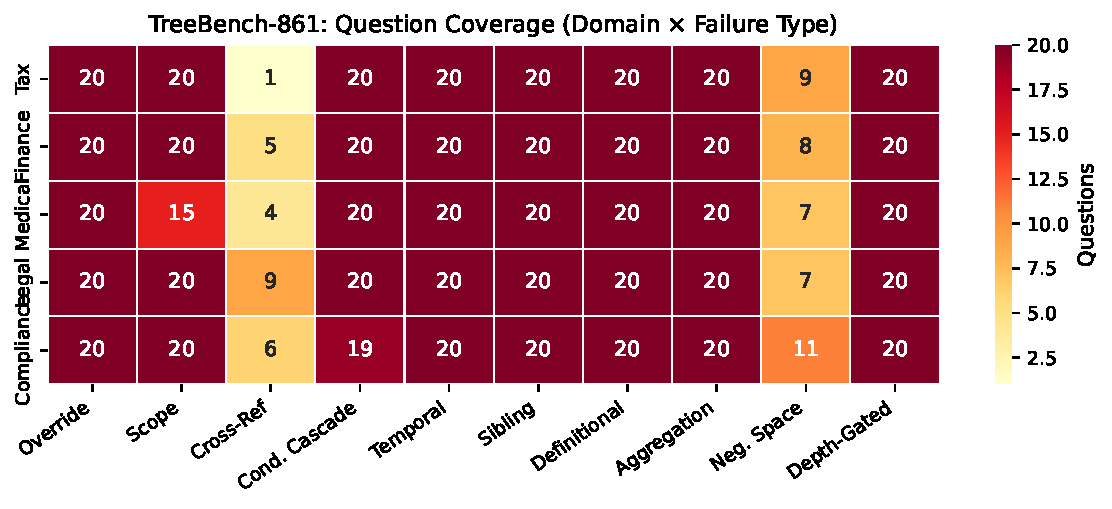
\includegraphics[width=\textwidth]{figures/fig2_coverage_heatmap.pdf}
\caption{Question coverage across the 5 $\times$ 10 grid of domains and failure types. Most cells reach the target of 20 questions; cross-reference and negative space have fewer candidates due to rarer structural patterns in the source corpus.}
\label{fig:coverage}
\end{figure*}

\begin{table}[h]
\centering
\small
\begin{tabular}{lc}
\toprule
\textbf{Validation Check} & \textbf{Result} \\
\midrule
Unique question IDs & \checkmark~Pass (861/861) \\
Required/distractor node overlap & 0 \\
Empty gold evidence & 0 \\
Duplicate question text & 0 \\
Signal hallucination (fabricated refs) & 0 \\
Mid-word evidence truncation & 0 \\
Structural giveaways in question & 0 \\
Oracle upper bound (acc / recall) & 100\% / 100\% \\
Domain $\times$ type cells covered & 50 / 50 \\
Candidates rejected during validation & 61 / 922 \\
\bottomrule
\end{tabular}
\caption{Automated validation results for TreeBench-861. All checks pass; 61 candidates were rejected during gold promotion for quality violations.}
\label{tab:validation}
\end{table}


% ════════════════════════════════════════════════════════════════════
\section{Evaluation Metrics}
\label{sec:metrics}

Standard retrieval evaluation relies on answer accuracy or passage-level recall. These metrics are insufficient for hierarchy-sensitive corpora because a system can produce a correct answer from the wrong evidence. We define four primary metrics:

\paragraph{Answer Accuracy.} Whether the system's answer matches the gold answer (exact match or semantic equivalence via LLM judge). This is the standard metric necessary but insufficient.

\paragraph{Path Accuracy.} Whether the system identifies the correct path through the tree hierarchy to the authoritative provision. A system scores 1.0 if its retrieved nodes include at least one node on the gold path.

\paragraph{Required-Node Recall.} The fraction of required evidence nodes that appear in the system's retrieved context: $\text{Recall} = |R_{\text{retrieved}} \cap R_{\text{required}}| / |R_{\text{required}}|$. This is our primary structural metric. A score below 1.0 means the system lacks complete authority evidence, even if it answers correctly.

\paragraph{Distractor Hit Rate.} The fraction of distractor nodes that appear in the retrieved context. High distractor hits indicate the system is selecting structural confounders semantically similar but positionally incorrect nodes.

We additionally report cost per query and latency for practical comparison.


% ════════════════════════════════════════════════════════════════════
\section{Baseline Methods}
\label{sec:baselines}

We evaluate 8 methods organized in two phases.

\subsection{Phase 1: Retrieval-Only Baselines}

\paragraph{Oracle.} Returns the gold required nodes directly. Establishes the upper bound and verifies that the scoring pipeline is correct (100\% on all metrics by construction).

\paragraph{BM25.} Lexical retrieval using BM25 scoring over all nodes in the relevant title. Returns top-10 nodes by BM25 score.

\paragraph{Dense RAG.} Embedding-based retrieval \cite{karpukhin2020dense} using sentence-transformers \cite{reimers2019sentencebert} (\texttt{all-MiniLM-L6-v2} \cite{wang2020minilm}). Returns top-10 nodes by cosine similarity to the query embedding.

\paragraph{Hybrid RAG.} Reciprocal rank fusion of BM25 and dense retrieval scores, combining lexical and semantic signals.

\paragraph{Reranker RAG.} Dense retrieval followed by cross-encoder reranking (\texttt{cross-encoder/ms-marco-MiniLM-L-6-v2}). Returns top-10 after reranking an initial pool of 50 candidates.

\subsection{Phase 2: LLM Reasoning Baselines}

These methods use GPT-4.1-mini as the reasoning model, applied over Dense RAG's retrieved context.

\paragraph{RAG + Chain-of-Thought.} The LLM receives the top-10 dense-retrieved nodes and is prompted to reason step-by-step about which provision is authoritative before answering.

\paragraph{RAG + Judge.} Two-stage: first, Dense RAG produces an answer; then a separate LLM call evaluates whether the answer is supported by the retrieved evidence, with the option to abstain.

\paragraph{Tree Traversal (naive).} The LLM navigates the tree top-down, choosing which child to expand at each level based on the query, without access to pre-retrieved nodes. This intentionally naive baseline tests whether an LLM can perform structure-aware navigation without any retrieval assistance.


% ════════════════════════════════════════════════════════════════════
\section{Results}
\label{sec:results}

\subsection{Main Results}

Table~\ref{tab:main} presents the main results across all 8 methods.

\begin{table*}[t]
\centering
\small
\begin{tabular}{llcccccc}
\toprule
& \textbf{Method} & \textbf{Accuracy} & \textbf{Path Acc.} & \textbf{Recall} & \textbf{Distr.} & \textbf{Cost/q} & \textbf{Latency} \\
\midrule
\multirow{5}{*}{\rotatebox{90}{\scriptsize Phase 1}}
& Oracle & 100.0\% & 100.0\% & 100.0\% & 0.00 & \$0.000 & 0.0s \\
& BM25 & 76.0\% & 87.7\% & 45.1\% & 0.22 & \$0.000 & 24.4s \\
& Hybrid RAG & 75.4\% & 87.3\% & 44.1\% & 0.27 & \$0.000 & 67.0s \\
& Dense RAG & 53.1\% & 70.3\% & 34.1\% & 0.15 & \$0.000 & 38.9s \\
& Reranker RAG & 34.5\% & 47.2\% & 21.2\% & 0.11 & \$0.000 & 114.9s \\
\midrule
\multirow{3}{*}{\rotatebox{90}{\scriptsize Phase 2}}
& RAG + CoT & 71.8\% & 70.3\% & 34.1\% & 0.15 & \$0.001 & 4.1s \\
& RAG + Judge & 56.8\% & 70.3\% & 34.1\% & 0.15 & \$0.002 & 6.2s \\
& Tree Traversal & 2.0\% & 2.4\% & 1.0\% & 0.00 & \$0.000 & 1.2s \\
\bottomrule
\end{tabular}
\caption{Main results on TreeBench-861. Recall = required-node recall. Distr.\ = distractor hit rate. Phase 2 methods use GPT-4.1-mini. RAG + CoT and RAG + Judge operate over Dense RAG's retrieved context, inheriting its recall ceiling.}
\label{tab:main}
\end{table*}

\subsection{Key Findings}

\paragraph{Finding 1: Accuracy masks structural failure.} BM25 achieves 76\% answer accuracy but only 45\% required-node recall. This means that for more than half of questions, the system produces an answer without complete structural authority evidence. In regulated domains, an answer without traceable authority is potentially non-compliant regardless of its surface correctness.

\paragraph{Finding 2: Dense retrieval is weaker than lexical.} Dense RAG (53\% accuracy, 34\% recall) substantially underperforms BM25 (76\% accuracy, 45\% recall). This is consistent with our hypothesis: embedding similarity conflates semantically related but structurally distinct nodes. The regulatory text reuses vocabulary extensively across hierarchical levels, creating embedding-space collisions that lexical matching partially avoids.

\paragraph{Finding 3: Reranking amplifies confounders.} In our evaluated setting, the reranker achieves only 34.5\% accuracy and 21\% recall the worst retrieval-only method. Cross-encoder reranking optimizes for query-passage relevance, which in hierarchical corpora can select \emph{against} authority. The confounder node is topically relevant (high reranker score) but positionally wrong.

\paragraph{Finding 4: Reasoning cannot fix upstream retrieval failure.} RAG + CoT achieves 72\% accuracy (slightly below BM25's 76\%) but identical recall to Dense RAG (34\%). The LLM can improve answer quality given the same context, but it cannot recover evidence nodes that were never retrieved. This demonstrates that the failure mode is in \emph{context selection}, not in reasoning capability.

\paragraph{Finding 5: Verification does not recover missing authority.} RAG + Judge (57\% accuracy, 34\% recall) performs \emph{worse} than CoT on accuracy while maintaining identical recall. The judge can identify some wrong answers but cannot determine that the retrieved evidence lacks structural authority it has no access to what \emph{should} have been retrieved.

\paragraph{Finding 6: Naive structure-aware navigation is hard.} Our naive tree traversal baseline achieves only 2\% accuracy. Top-down navigation through regulatory trees requires understanding which branch contains the authoritative provision at each level a capability current LLMs lack in this domain without additional scaffolding.

\begin{figure*}[t]
\centering
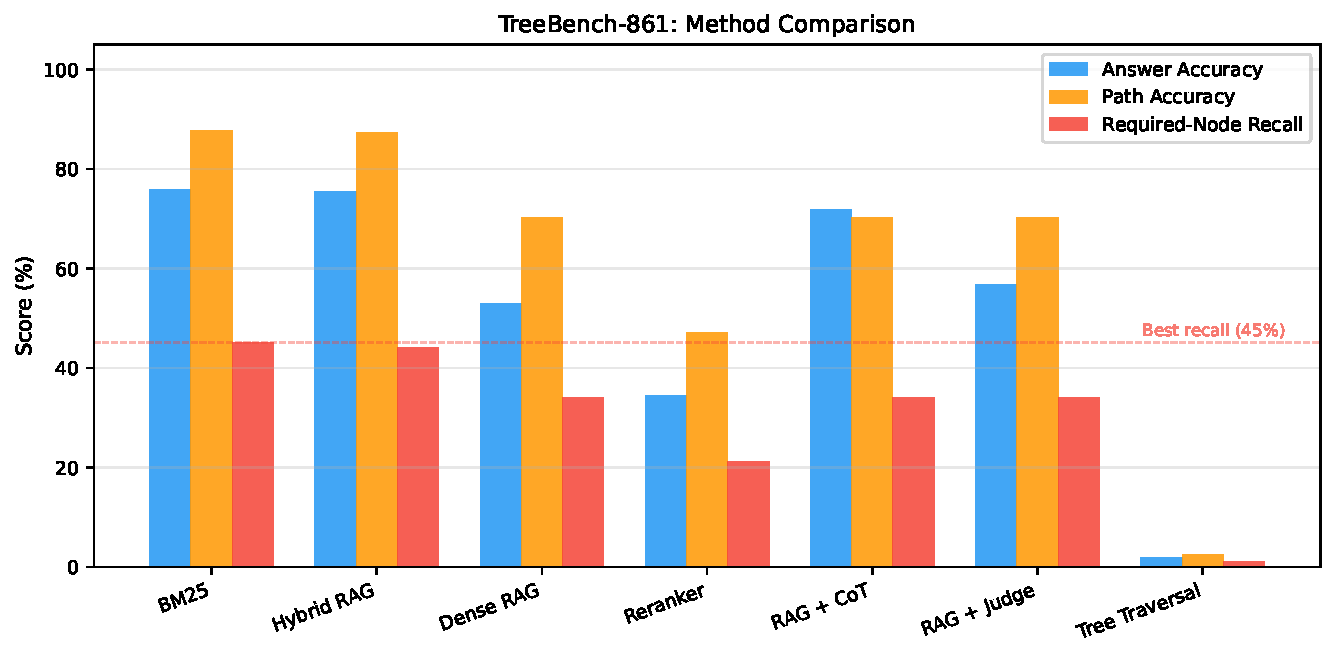
\includegraphics[width=\textwidth]{figures/fig5_baseline_bars.pdf}
\caption{Method comparison across three metrics. The gap between answer accuracy (blue) and required-node recall (red) is visible for every method. The dashed line marks the best non-oracle recall (45\%).}
\label{fig:baseline_bars}
\end{figure*}

\subsection{Breakdown by Failure Type}

Table~\ref{tab:failure_breakdown} shows how different failure types challenge the best retrieval method (BM25).

\begin{table}[h]
\centering
\small
\begin{tabular}{lcc}
\toprule
\textbf{Failure Type} & \textbf{Accuracy} & \textbf{Recall} \\
\midrule
Conditional Cascade & 92.9\% & 48.5\% \\
Scope Disambiguation & 88.4\% & 33.9\% \\
Sibling Conflict & 84.0\% & 65.0\% \\
Definitional Dependency & 84.0\% & 50.0\% \\
Override Chain & 77.0\% & 31.5\% \\
Temporal Layering & 76.0\% & 49.5\% \\
Aggregation & 74.0\% & 55.2\% \\
Depth-Gated Specificity & 69.0\% & 48.0\% \\
Cross-Reference & 52.0\% & 34.7\% \\
Negative Space & 2.4\% & 1.2\% \\
\bottomrule
\end{tabular}
\caption{BM25 performance by failure type, sorted by accuracy. Negative space (``no provision exists'') is nearly impossible for retrieval systems designed to \emph{find} matches.}
\label{tab:failure_breakdown}
\end{table}

Notable patterns:
\begin{itemize}[nosep]
    \item \textbf{Scope disambiguation} shows the largest accuracy-recall gap (88\% vs.\ 34\%): the system often guesses correctly from partial context but retrieves the wrong scope's definition.
    \item \textbf{Negative space} is catastrophic (2.4\% accuracy): retrieval systems are fundamentally designed to return results, making ``nothing applies'' nearly impossible to conclude.
    \item \textbf{Override chain} has low recall (31.5\%) despite moderate accuracy (77\%): systems find the general rule but miss the overriding exception.
    \item \textbf{Sibling conflict} has the highest recall (65\%) because both conflicting provisions share vocabulary and tend to be co-retrieved.
\end{itemize}


% ════════════════════════════════════════════════════════════════════
\section{Analysis}
\label{sec:analysis}

\begin{figure*}[t]
\centering
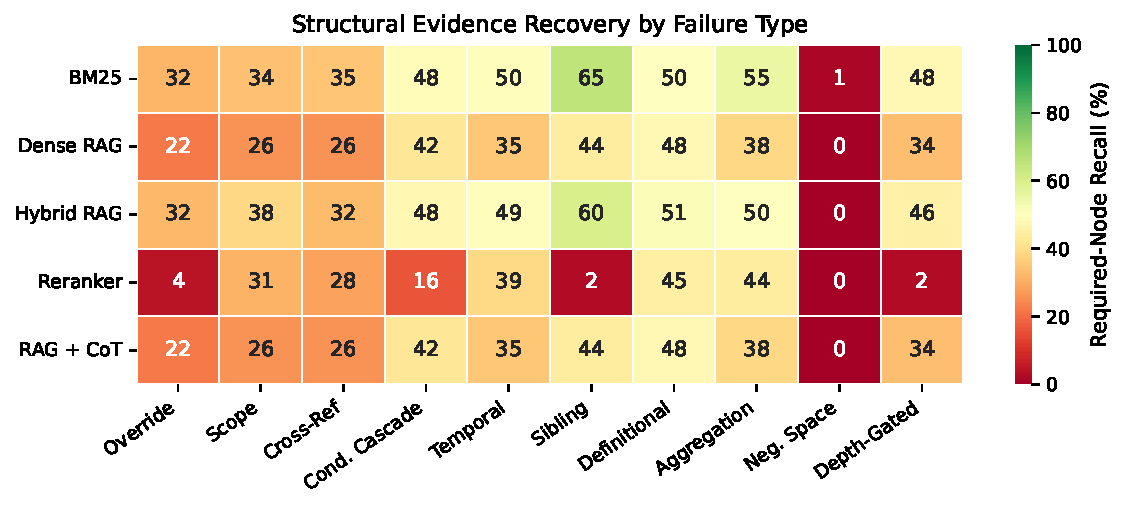
\includegraphics[width=\textwidth]{figures/fig4_recall_heatmap.pdf}
\caption{Required-node recall by failure type across retrieval methods. Negative space is catastrophic (0\% recall) for all methods. Reranking shows near-zero recall on override chains and depth-gated specificity, confirming confounder amplification.}
\label{fig:recall_heatmap}
\end{figure*}

\subsection{The Authority Gap}

We define the \textbf{authority gap} as the difference between answer accuracy and required-node recall for a given method (Figure~\ref{fig:authority_gap}). This gap measures how often a system produces answers without complete structural justification:

\begin{center}
\small
\begin{tabular}{lc}
\toprule
\textbf{Method} & \textbf{Authority Gap} \\
\midrule
BM25 & 30.9 pp \\
Hybrid RAG & 31.3 pp \\
RAG + CoT & 37.7 pp \\
Dense RAG & 19.0 pp \\
RAG + Judge & 22.7 pp \\
Reranker & 13.3 pp \\
\bottomrule
\end{tabular}
\end{center}

The largest authority gaps occur in methods that achieve high accuracy: BM25 and Hybrid RAG answer many questions ``correctly'' without retrieving complete evidence. RAG + CoT has the largest gap overall (37.7 pp), indicating that reasoning amplifies the appearance of correctness while the evidence foundation remains unchanged.

\begin{figure}[h]
\centering
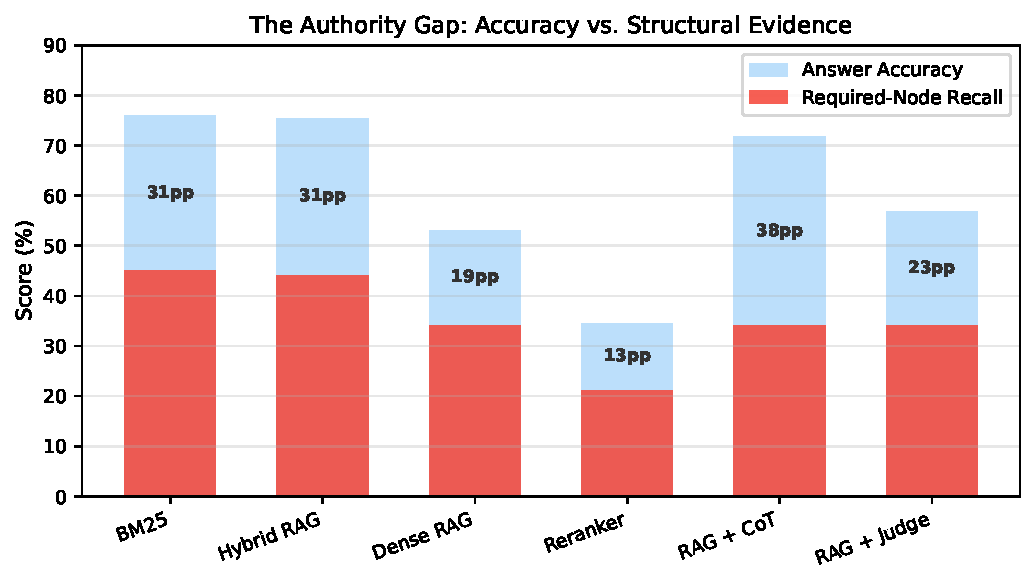
\includegraphics[width=\columnwidth]{figures/fig6_authority_gap.pdf}
\caption{The authority gap: difference between answer accuracy and required-node recall. RAG + CoT has the largest gap (38 pp) reasoning improves surface answers without improving evidence quality.}
\label{fig:authority_gap}
\end{figure}

\subsection{Why Reranking Fails}

Cross-encoder rerankers are trained to score query-passage relevance on datasets like MS MARCO where any passage containing the answer is valid evidence. In hierarchical corpora, this objective is misaligned: the structural confounder is \emph{maximally relevant} to the query (it discusses the same topic, uses the same terms) but is not \emph{authoritative} (it occupies the wrong position in the hierarchy). The reranker assigns high scores to confounders precisely because they are topically relevant, pushing authoritative but less obviously relevant nodes out of the top-$k$.

\subsection{Implications for Deployed Systems}

In regulated industries (finance, healthcare, tax), retrieval systems are increasingly used to provide authoritative answers to compliance questions. Our findings suggest that:

\begin{enumerate}[nosep]
    \item Answer accuracy benchmarks overstate the reliability of these systems by 30+ percentage points.
    \item Post-hoc reasoning (CoT) and verification (judge) provide false confidence: they improve answer formatting without improving evidence quality.
    \item The failure mode is systematic, not random: it specifically targets the structural authority relationships that make regulatory text legally binding.
\end{enumerate}


% ════════════════════════════════════════════════════════════════════
\section{Discussion and Limitations}
\label{sec:discussion}

\paragraph{Scope.} TreeBench currently covers U.S.\ federal regulations (eCFR). Other hierarchical corpora (case law, international treaties, corporate policies) may exhibit different structural patterns. We believe the failure taxonomy generalizes but have not empirically validated this.

\paragraph{Question generation.} Questions are generated by an LLM from mined structural patterns, not written by domain experts. While we apply extensive automated validation (structural giveaway detection, signal verification, overlap checking), some questions may not perfectly mirror how practitioners phrase regulatory queries.

\paragraph{Partial coverage.} Not all 50 cells (5 domains $\times$ 10 failure types) reach the target of 20 questions; cross-reference (25 total) and negative space (42 total) have fewer candidates due to rarer structural patterns. This reflects genuine variation in how failure types manifest across domains.

\paragraph{Retrieval scope.} Each question is evaluated against the nodes of its source eCFR title (tens of thousands of nodes), not the full 591,793-node corpus. This is a deliberate design choice that isolates structural authority failures from corpus-scale retrieval noise. Retrieval over the full corpus would likely produce lower scores across all methods.

\paragraph{Baseline scope.} We evaluate representative methods using widely available models (all-MiniLM-L6-v2, ms-marco-MiniLM-L-6-v2, GPT-4.1-mini) but do not test all possible configurations. Larger embedding models (e.g., text-embedding-3-large), stronger rerankers (e.g., Cohere rerank-3), and frontier reasoning models may narrow the gap. If the failure is genuinely structural, it should persist with stronger models; we leave this verification to future work. Results are single-run without confidence intervals; the LLM-based methods (CoT, Judge, Tree Traversal) are stochastic. TreeBench is released as a benchmark and we expect future work to develop methods that better address structural authority.

\paragraph{Tree traversal.} Our tree traversal baseline is intentionally naive (single-pass top-down). More sophisticated approaches (beam search, backtracking, multi-step planning) may perform substantially better and represent a promising research direction.

\paragraph{Reproducibility.} We release the following artifacts at \url{https://github.com/whitepaper27/TreeBench}, following dataset documentation best practices \cite{gebru2021datasheets}:
\begin{enumerate}[nosep]
    \item The 861-question gold dataset with required/distractor node IDs
    \item Automated validation report (all quality checks)
    \item Source code for tree parsing, failure-pattern mining, and question generation
    \item All baseline evaluation scripts (BM25, Dense, Hybrid, Reranker, CoT, Judge, Tree Traversal)
    \item Baseline results and per-question evaluation outputs
\end{enumerate}
We encourage future work to report structural evidence metrics (required-node recall, distractor hit rate) alongside accuracy when evaluating retrieval over hierarchically organized corpora.


% ════════════════════════════════════════════════════════════════════
\section{Conclusion}
\label{sec:conclusion}

We introduced TreeBench, a benchmark that exposes structural evidence failures in retrieval over hierarchical corpora. Our evaluation of 8 methods reveals a consistent finding: \textbf{similarity is not authority}. Systems achieve moderate response accuracy, while systematically failing to recover the structural evidence that makes these answers defensible.

The best non-oracle method reaches only 45\% required-node recall. Chain-of-thought reasoning and LLM-based verification do not address this gap because the failure occurs upstream of reasoning---in the selection of which evidence to reason over. In our setting, reranking---designed to improve retrieval quality---worsens it by amplifying structural confounders.

We release TreeBench-861 as an open challenge to the retrieval community. Solving hierarchical authority selection will require methods that go beyond similarity, incorporating tree position, scope relationships, and structural metadata into the retrieval process itself.


% ════════════════════════════════════════════════════════════════════
\section*{Acknowledgments}

The author thanks the maintainers of public regulatory and statutory data sources, including the electronic Code of Federal Regulations and related U.S. government open-data resources, whose structured public documents made this benchmark possible. The author also acknowledges the open-source software ecosystem used in this work, including Python, NumPy, Matplotlib, Seaborn, and retrieval/evaluation tooling used to construct and analyze TreeBench.

Commercial large language model APIs were used in selected baseline experiments and as research assistance tools for drafting, refactoring, and experimental workflow support. These systems were used only as tools; they did not determine the benchmark labels, validation criteria, experimental interpretation, or final claims. All benchmark design decisions, data set validation, and conclusions remain the authors' responsibility.

No external funding was received for this work.

% ════════════════════════════════════════════════════════════════════
\bibliographystyle{plainnat}
\bibliography{references}

\end{document}
